\documentclass[10pt, compress]{beamer}
\usetheme[conference=MST1-TFM,venue=Padova, date=23/05/2018, titleprogressbar, logo=RFX-logo]{Eurof}
\usepackage{listings,amsmath,multimedia, amssymb}
\usepackage{tangocolors}
\usepackage{rfxcolor}
\definecolor{colorA}{HTML}{324D5C}
\definecolor{colorB}{HTML}{E37B40}
\definecolor{colorC}{HTML}{60A65F}

% for drawing
\usepackage{pgf}
\usepackage{tikz}
\usetikzlibrary{arrows,shapes,backgrounds}
\usepackage{onimage}
\usepackage[export]{adjustbox}
% for font
\usepackage[absolute,overlay]{textpos}
  \setlength{\TPHorizModule}{1mm}
  \setlength{\TPVertModule}{1mm}

\usepackage[style=nature,citestyle=authoryear-comp,defernumbers=true,maxnames=2,firstinits=true,
uniquename=init,backend=bibtex8,arxiv=abs,mcite]{biblatex}
\bibliography{../biblio}
\renewcommand*{\bibfont}{\footnotesize}
\renewcommand*{\citesetup}{\footnotesize}
\usepackage[export]{adjustbox}
\makeatother
\mode<presentation>
\makeatletter
% add a macro that saves its argument
\newcommand{\footlineextra}[1]{\gdef\insertfootlineextra{#1}}
\newbox\footlineextrabox
% for reducing font on a single slide
\newcommand\Fontvi{\fontsize{8}{7.2}\selectfont}
\title{Filamentary transport in high-power H-mode conditions and in no/small-ELM regimes to predict heat and particle loads on PFCs for future devices}
\date{23 May 2018}
\author[N.Vianello]{presented by N. Vianello on behalf of  MST1-Topic 21
  scientific team}
\begin{document}
\tikzstyle{every picture}+=[remember picture]
\maketitle
\begin{frame}{Scientific team}
  \centering{
  Volker Naulin, Matteo Agostini, Diogo Aguiam, Scott Allan, Matthias Bernert, Daniel Carralero Ortiz, 
Stefan Costea, Istvan Cziegler, Hugo De Oliveira, Joaquin Galdon-Quiroga, Gustavo Grenfell, Antti Hakola, 
Codrina Ionita-Schrittwieser, Heinz Isliker, Alexander Karpushov,
Jernej Kovacic, Benoît Labit, Bruce Lipschultz, 
Roberto Maurizio, Ken McClements, Fulvio Militello, Jeppe Miki Busk Olsen, Jens Juul Rasmussen, Timo Ravensbergen, Bernd Sebastian Schneider, Roman Schrittwieser, Jakub Seidl, Monica Spolaore, Christian Theiler, Cedric Kar-Wai Tsui, Kevin Verhaegh, Jose Vicente, 
Nickolas Walkden, Zhang Wei, Elisabeth Wolfrum, W. Vijvers}
\end{frame}

\begin{frame}{Background}
  \only<1>{
\begin{itemize}
\item Role of turbulence transport in the SOL saturation is a well
  know
  feature \parencite{LaBombard:2001ks,Rudakov:2005ic,Garcia:2007hh,Carralero:2014gs}. \textcolor{red}{Increasing
  density, even without reaching detachment SOL profile tend to flatten}
\end{itemize}}
% \only<2-3>{
%   \begin{columns}
%     \begin{column}{0.5\textwidth}
%       \begin{itemize}
%       \item Present understanding suggests that a transition of filament
%         propagation regime is dominated by effective
%         collisionality $\Lambda$ \parencite{Myra:2006p2754}
%         \begin{equation*}
%           \Lambda = \frac{L_{\parallel}/c_s}{1/\nu_{ei}}\frac{\Omega_i}{\Omega_e}
%         \end{equation*}
%         \item<3> \textcolor{red}{At constant blob size, increasing
%             collisionality provide a change in the filaments velocity
%             scaling properties}
%       \end{itemize}
%     \end{column}
%     \begin{column}{0.5\textwidth}
% %      \includegraphics<2>[width=\textwidth]{../pdfbox/Presentation/FigMyra}
%         \begin{tikzonimage}[width=\textwidth]{../generalFigures/FigMyra}
%           \only<3>{
%             \draw [->, ultra thick, red] (0.7,0.3) -- (0.7,0.6);}
%         \end{tikzonimage}
%     \end{column}
%   \end{columns}
% }
\only<2-4>{
  \begin{columns}
    \begin{column}{0.5\textwidth}
      \begin{itemize}
      \item AUG and JET (HT) \parencite{Carralero:2015gu} suggest that $\Lambda_{div}=\frac{L_{\parallel}/c_s}{1/\nu_{ei}}\frac{\Omega_i}{\Omega_e}$ dominates this
        process and a transition from
        \textcolor{ta3chameleon}{sheath-limited}
        \onslide<3-4>{to \textcolor{blue}{inertial regime}} 
        \item<4> \textcolor{red}{Tested by changing n$_e$
            and $T_e$ through fueling/seeding/heating}
      \end{itemize}
    \end{column}
    \begin{column}{0.5\textwidth}
      \begin{tikzonimage}[width=\textwidth]{../generalFigures/KoMFig2.png}
        \only<2-4>{
          \draw [thick, ta3chameleon, thick] (0.45,0.25) ellipse (0.23 and 0.1);
      }
        \only<3-4>{
          \draw [thick, blue, thick, rotate=-4] (0.8,0.55) ellipse (0.1 and 0.33);
      }
        \only<4>{
          \draw [thick, red, thick, dashed] (0.35,0.75) circle (0.25);
      }
    \end{tikzonimage}
  \end{column}
  \end{columns}
}
\only<5-7>{
  \begin{columns}[c]
    \begin{column}{0.4\textwidth}
      \begin{itemize}
      \item<5|only@5> $\Lambda_{div}$ does not describe properly evolution
        of upstream profile in JET-VT \parencite{Wynn:2018gp}
      \item<6-7> On TCV \parencite{Vianello:2017ku} $\Lambda_{div}$
        necessary but not sufficient to guarantee increase $\lambda_n$
        in the far SOL
      \item<7|only@7> Additional mechanism suggested among which
        \alert{neutral clogging} 
    \end{itemize}
  \end{column}
  \begin{column}{0.6\textwidth}
    \centering{\includegraphics<5>[width=\textwidth]{../generalFigures/Wynn-HT-VT}}
    \centering{\includegraphics<6-7>[width=\textwidth]{../generalFigures/Vianello-TCV}}
  \end{column}
\end{columns}
}
\centering{\includegraphics<1>[width=1.1\textwidth]{../generalFigures/Various-density-profiles}}
\end{frame}

\begin{frame}{Motivation and deliverables}
  \Fontvi
  \vspace{-1cm}
  \begin{itemize}
    \item \alert{Relation between downstream divertor conditions and
        up-stream SOL profiles is not well understood. Influence of
        SOL blob structures on shoulder formation and divertor
        conditions is key element towards predictive
        capabilities. Joint effort within the EUROfusion framework to
        address this issue on all the MST1 devices (AUG, TCV and MAST-U)}
  \end{itemize}
  \onslide<2->{A series of deliverables were foreseen by 2017 program
\begin{enumerate}
\item \only<3>{\color{ta3chameleon}} Cross-machine L-Mode
  shoulder dependence on current both at constant B$_t$ and at
  constant $q_{95}$. Rationale: disentangle the effect of current and
  parallel connection length
\item \only<3>{\color{ta3chameleon}}Establish robust scenario for density
  shoulder profile in H-Mode and \only<3>{\color{ta3orange}}establish dependence on
  fuelling/neutral profiles/divertor condition
\item \only<3>{\color{ta3chameleon}}Fluctuations mesurement on AUG to study
  filamentary transport under high-power H-Mode conditions \only<3>{\color{ta2plum}}and under
  different plasma configurations (SN, DN)
\item \only<3>{\color{ta3orange}}Study the role of ELM regimes,  neutral
  compression and particle density in filamentary transport and
  related shoulder formation
\item \only<3>{\color{ta3orange}} Identify the contribution of
  collisionality and seeding on filamentary transport and related
  shoulder formation
\item \only<3>{\color{ta3orange}}Determine the effect of filaments and
  shoulder formation on target heat loads \only<3>{\color{ta2plum}}in different H-mode plasmas
\end{enumerate}}
\onslide<3>{
\textcolor{red}{Remember this is
  still a work in progress}
}
\end{frame}

\begin{frame}{Devices, diagnostics and methods}
\only<1>{
  \centering{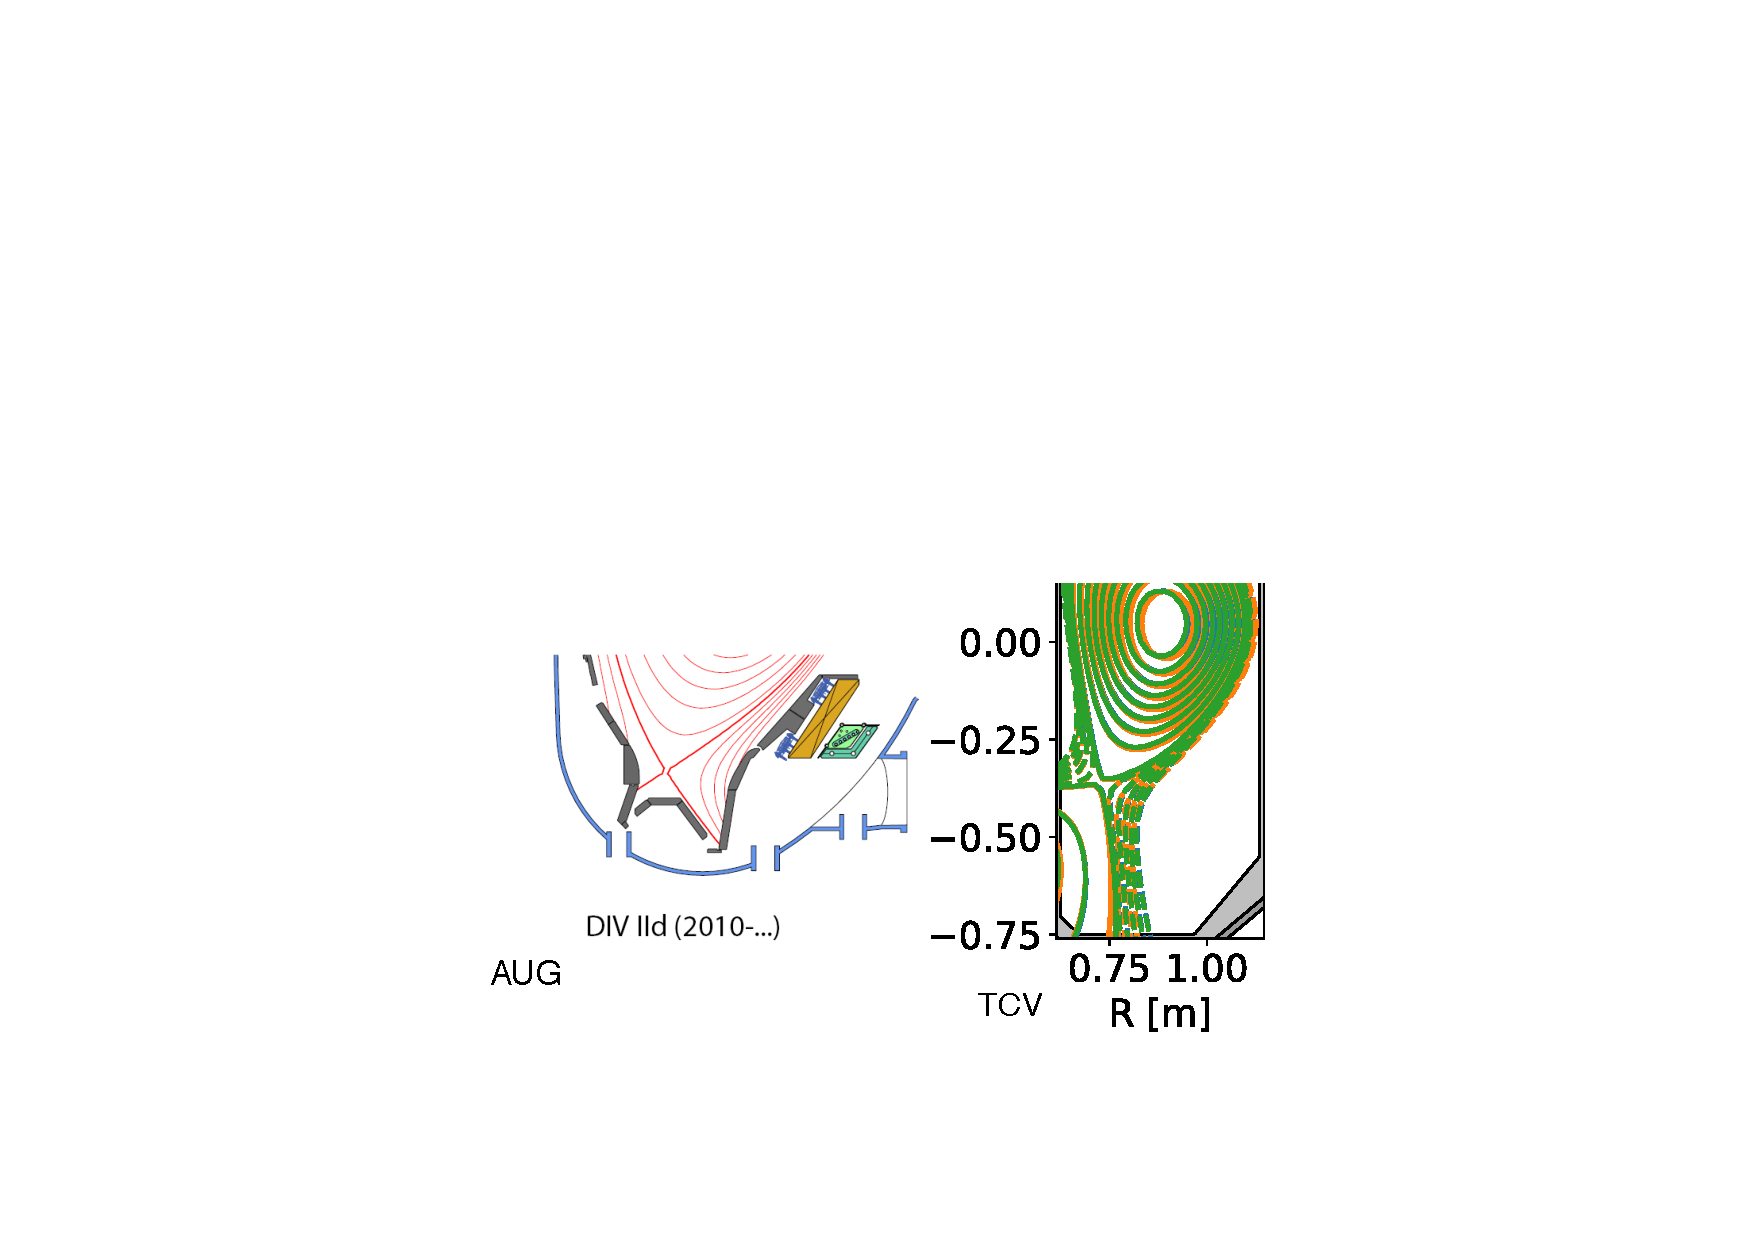
\includegraphics[width=0.8\textwidth]{../generalFigures/Divertor-AUG-TCV}}

  \begin{itemize}
    \item \textbf{AUG:} Metallic wall, cryopumps, closed divertor with
      SP on vertical target, short divertor leg
    \item \textbf{TCV:} Carbon wall, completely open divertor,
      operated with relative long divertor leg, no cryopump  
  \end{itemize}
}
\only<2>{
  \vspace{-1.5cm}
  \centering{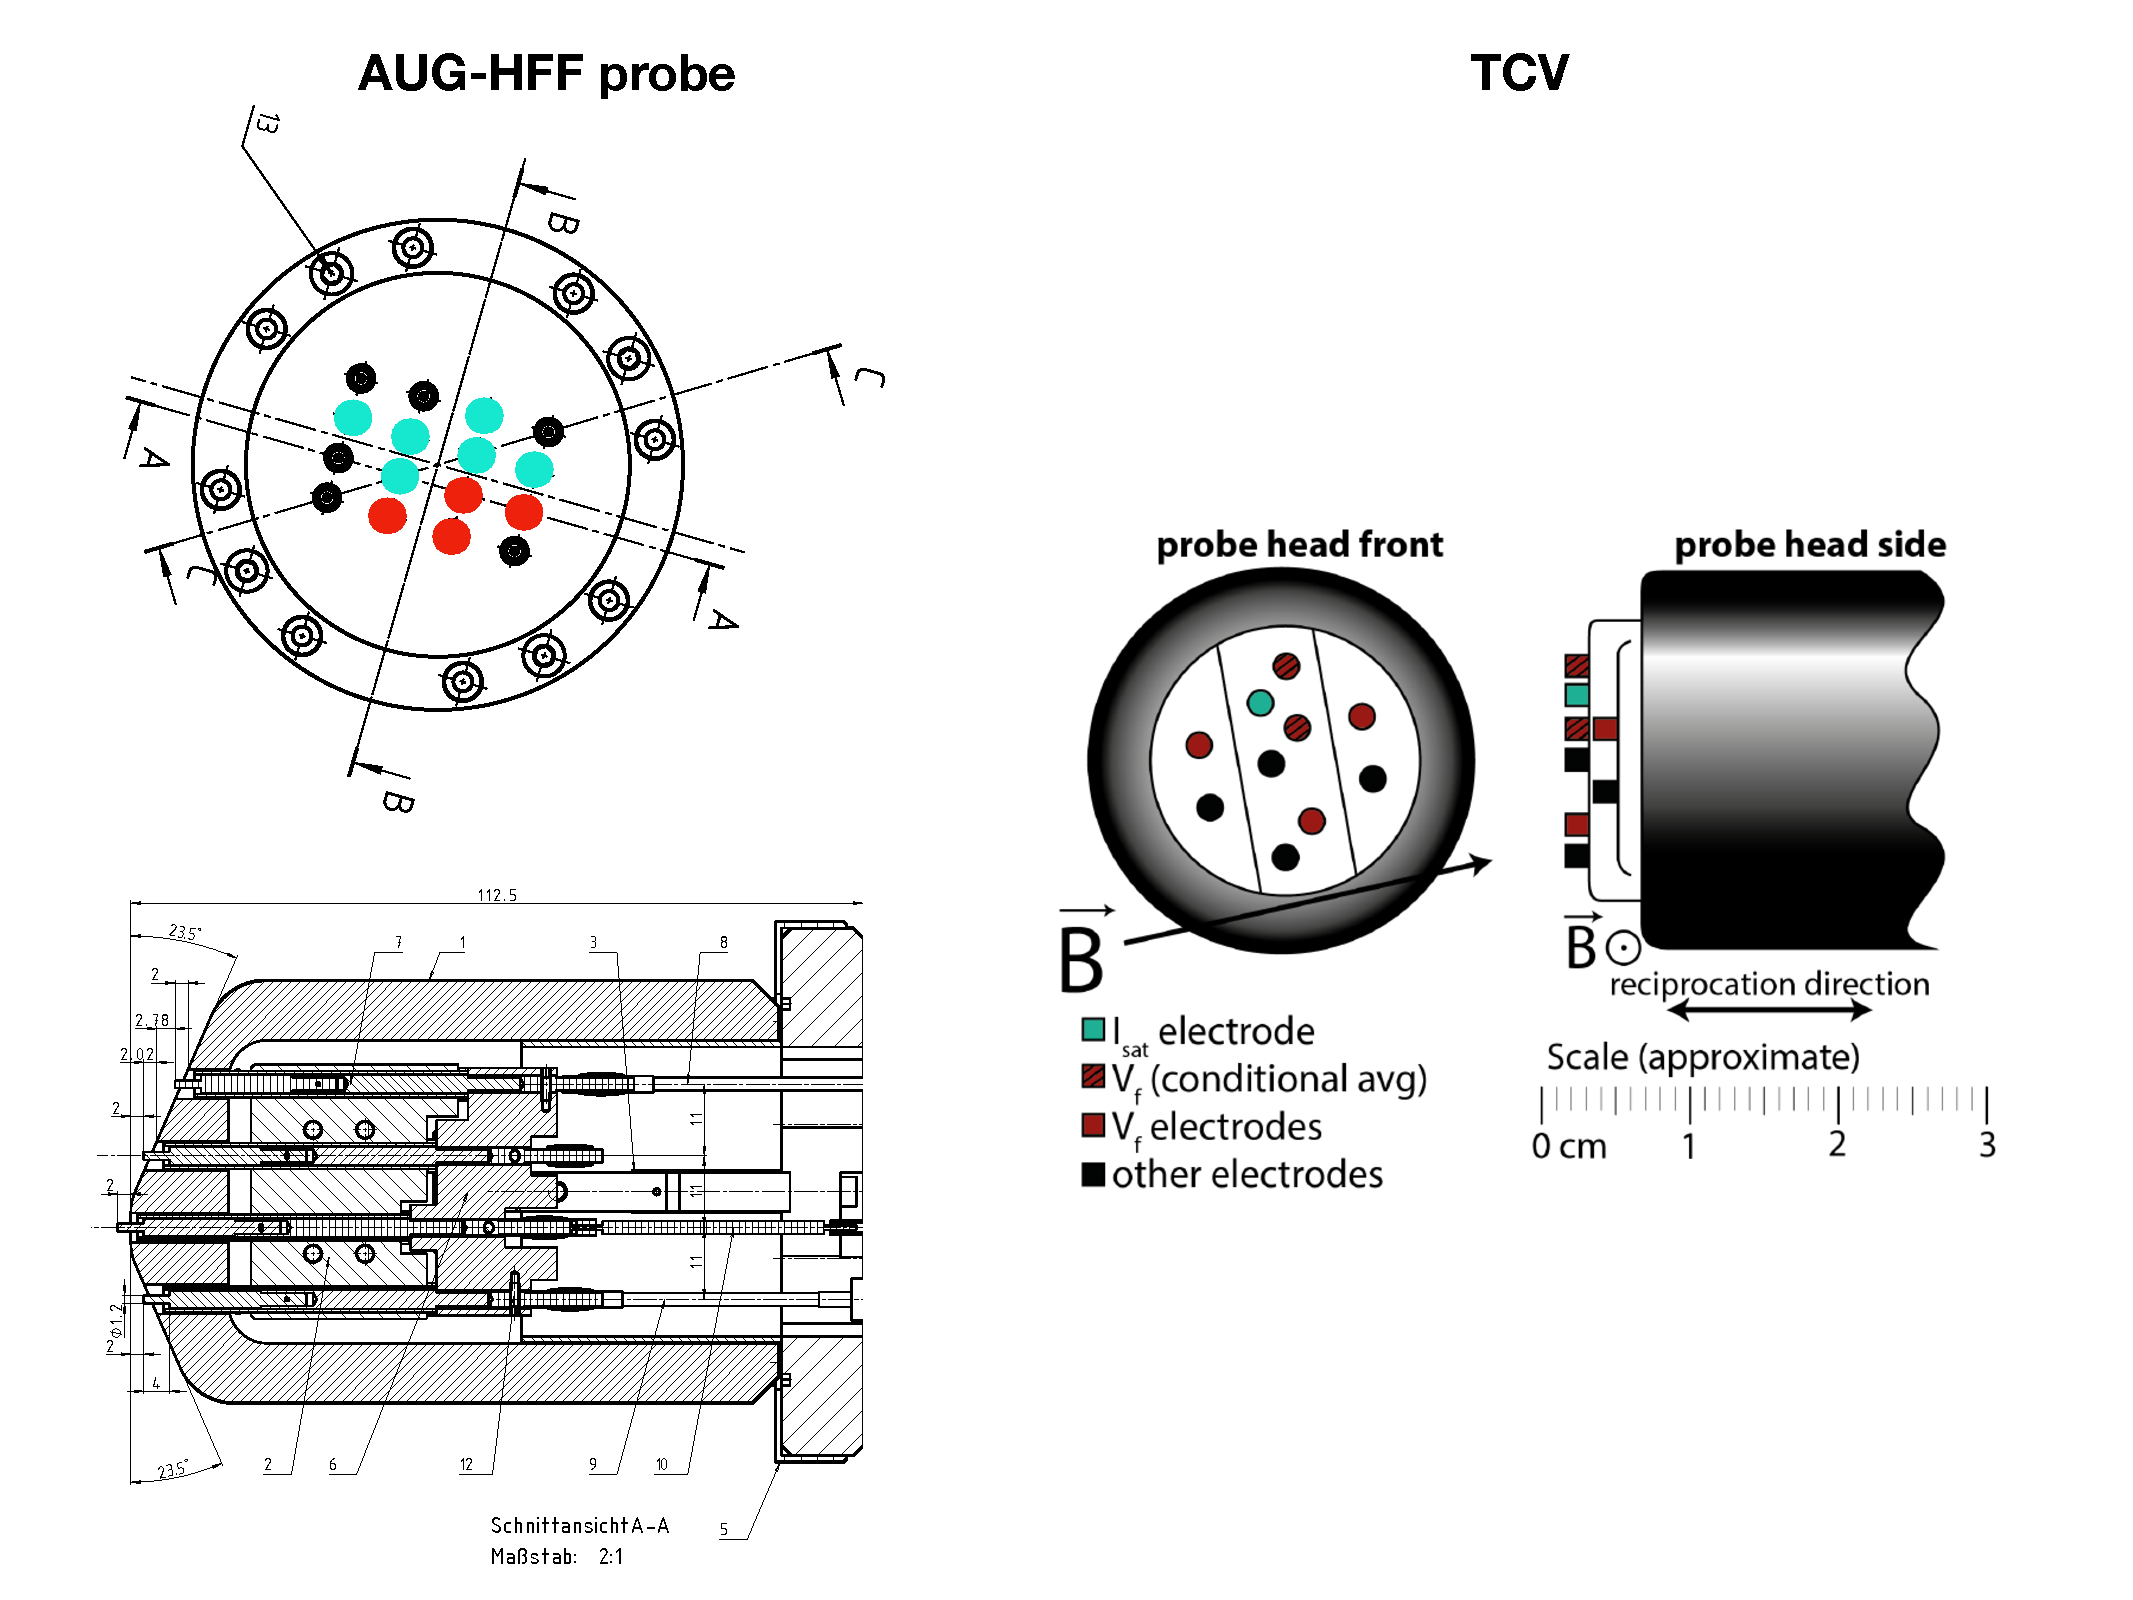
\includegraphics[width=0.7\textwidth]{../generalFigures/ProbeHead}}
\Fontvi
  \begin{itemize}
    \item \textbf{AUG:} Ion saturation current measured at different
      radial/poloidal position to get velocity from 2D cross-correlation
    \item \textbf{TCV:} Only 1 j$_{sat}$ measurement available,
      different velocity estimate. $v_r$ from
      $\mathbf{E}\times\mathbf{B}$ evaluation from floating potentials
      on CAS, $v_z$ from 2D cross-correlation analysis
  \end{itemize}
}
\only<3>{
  \centering{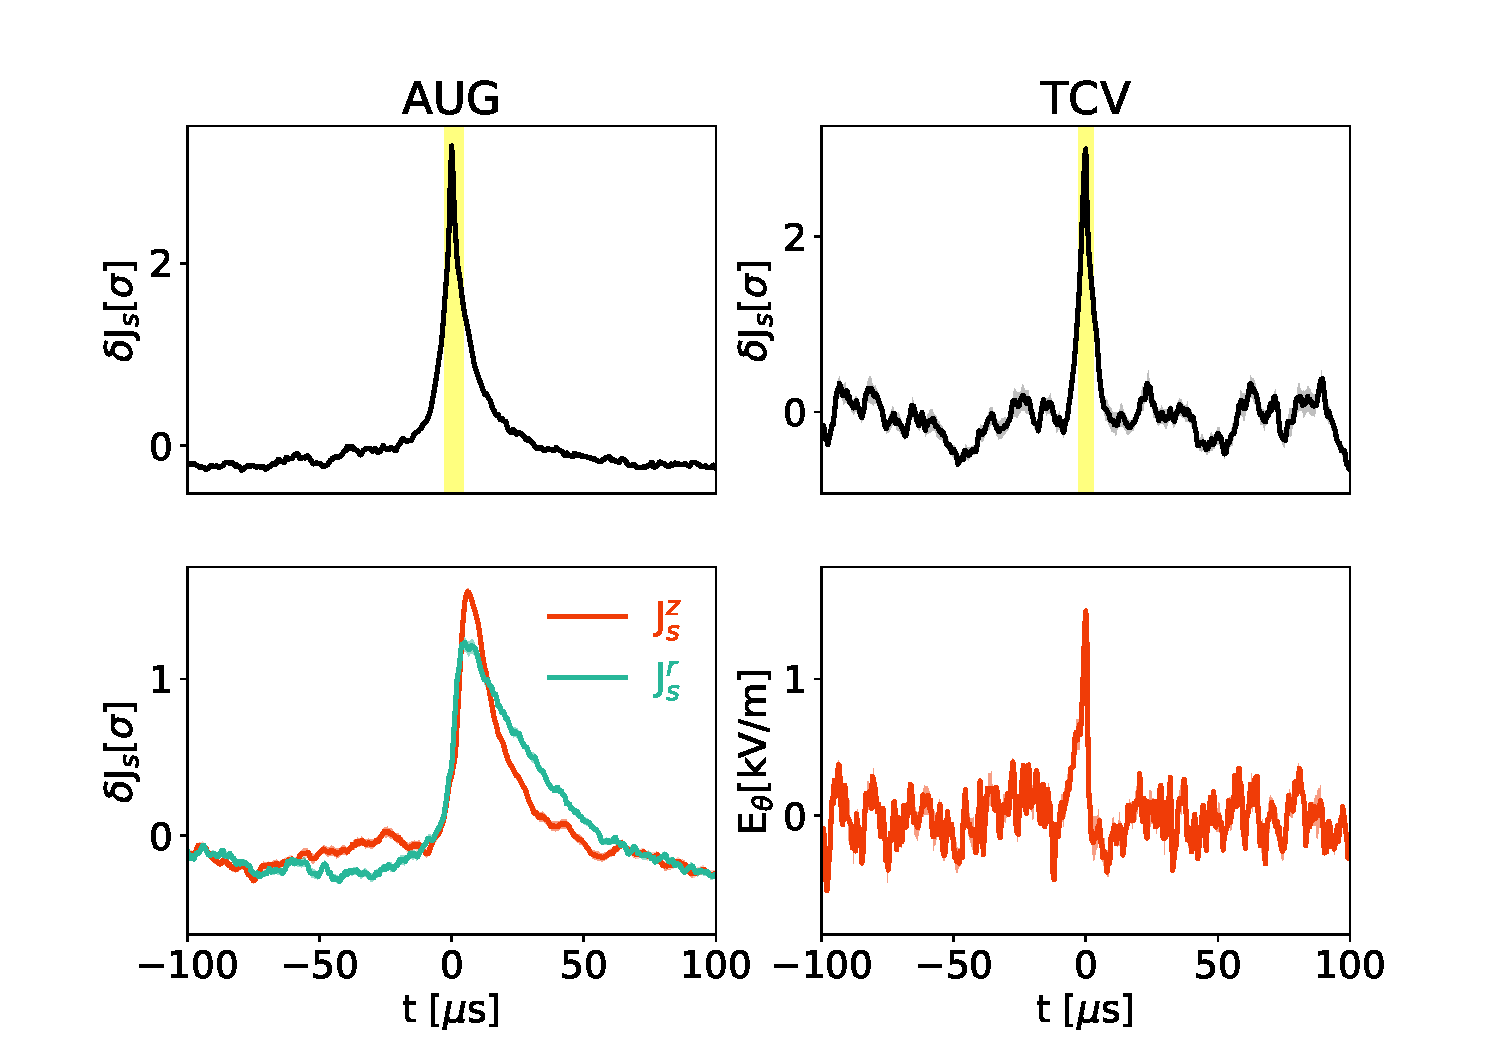
\includegraphics[width=0.7\textwidth]{../../Experiments/Comparison/pdfbox/ExampleCas}}
  \begin{itemize}
    \item Blob-size is $\delta_b = 0.5 * \tau_b*v_{\perp}$
    \item $\tau_b$ estimated from FWHM of Conditional Avearage
      binormal blob velocity estimated (although differently in the
      two devices)
  \end{itemize}
}
\end{frame}


\begin{frame}{Current scan at constant B$_t$ in L-Mode plasma}
  \begin{columns}
    \begin{column}{0.6\textwidth}
      \includegraphics<1>[width=\textwidth]{/Users/vianello/Documents/Fisica/Conferences/IAEA/iaea2018/pdfbox/EquilibriaIpScanConstantBt}
      \includegraphics<2>[width=\textwidth]{../../Experiments/AUG/analysis/pdfbox/GeneralIpScanConstantBt}
      \includegraphics<3>[width=.9\textwidth]{../../Experiments/TCV/analysis/pdfbox/CurrentScanConstantBt}
      \includegraphics<4>[width=\textwidth]{../../Experiments/Comparison/pdfbox/TargetDensityRadiationVsDensityConstantBt}
      \includegraphics<5>[width=\textwidth]{../../Experiments/Comparison/pdfbox/TargetDensityRadiationVsGreenwaldConstantBt}
      \only<6>{
        \begin{tikzonimage}[width=\textwidth]{../../Experiments/Comparison/pdfbox/TargetDensityRadiationVsDensityConstantBt}
          \draw [thick, ta3orange, ->] (0.27, 0.9) -- (0.27, 0.8);
          \draw [thick, ta3orange, ->] (0.77, 0.45) -- (0.77, 0.55);
        \end{tikzonimage}
      }
      \includegraphics<7>[width=\textwidth]{../../Experiments/Comparison/pdfbox/UpstreamTargetProfilesConstantBt}
      \includegraphics<8>[width=\textwidth]{../../Experiments/Comparison/pdfbox/ExampleShoulderAmplitude}
      \includegraphics<9>[width=\textwidth]{../../Experiments/Comparison/pdfbox/AmplitudeTargetVsDensityConstantBt}
      \includegraphics<10>[width=\textwidth]{../../Experiments/Comparison/pdfbox/AmplitudeTargetVsGreenwaldConstantBt}      
      \includegraphics<11>[width=\textwidth]{../../Experiments/Comparison/pdfbox/AmplitudeVsLambdaConstantBt}
      \includegraphics<12>[width=\textwidth]{../../Experiments/Comparison/pdfbox/EfoldBlobConstantBt}         
      \includegraphics<13>[width=\textwidth]{../../Experiments/Comparison/pdfbox/EfoldLambdaConstantBt}         
    \end{column}
    \begin{column}{0.4\textwidth}
      \begin{itemize}
        \item<1|only@1> Shape matched in within the single scan done for each of
          the machine
        \item<1|only@1> The scan implies a modification of the
          L$_{\parallel}$ (shown from the X-point height to the outer
          target).
          There is a factor of 5 difference between
          the two machines due to the very long outer divertor leg of TCV
        \item<2|only@2> AUG: Fueling reduced only at lower I$_p$ to
          avoid earlier disruption. Similar neutral pressure in the
          subdivertor region reached. 0.5 MW NBI additional power added to
          keep power in the SOL approximately constant
        \item<3|only@3> TCV: Ohmic heating only. Similar neutral compression reached and
          D$_{\alpha}$ radiation from the floor. Ion flux rollover
          reached in all the three current,  although marginally at
          330 kA
        \item<4|only@4> In both the machines both the peak target
          density and the radiation close to divertor target exhibit
          rollover at increasing density with increasing current
        \item<5|only@5> Whenever considered as a function of
          Greenwald fraction the behaviors at different currents
          almost reconciled for AUG \alert{but not for TCV and at 0.6
            MA for AUG}
        \item<only@6-7> We now consider the Target and upstream
          profiles at the same level of densities  
        \item<only@7> For both AUG and TCV flattening of normalized
          upstream profile reached \alert{earlier in density at lower
            current.} For both the machine the increase of $\lambda_n$
          reached for larger values of $\Lambda_{div}$
        \item<only@8> Quantifying profile evolution using the
          \alert{shoulder amplitude metric} introduce by Wynn and
          Lipschultz for JET \parencite{Wynn:2018gp}.
        \item<only@8>  \alert{Amplitude is the difference
            between normalized upstream density profiles}
        \item<only@8> Distinguishing behavior on the near and far SOL  
        \only<9-10>{\item Amplitude evolve faster in density at lower
          current in the far SOL. Amplitude starts increasing close to
          the transition to highly-recycling regime in analogy to
          JET HT \parencite{Wynn:2018gp} \onslide<10>{\alert{but once evolution \textit{vs} greenwald
            fraction is considered the evolution is equivalent between
            different current.}}
          \item<only@10> \textcolor{ta3chameleon}{Still some inconsistency at lower
            current in agreement with different detachment evolution}}
        \item<only@11> Amplitude evolution reconciled in AUG if
          considered as a function of local evolution of $\Lambda_{div}$
        \item<only@12> For both AUG and TCV $\lambda_n$ increases
          with blob size without significant difference within the
          current explored
        \item<only@13> \alert{The evaluation of $\lambda_n$ as a
          function of $\Lambda_{div}$ confirms that this variable is
          insufficient to completely reconcile AUG and TCV}
      \end{itemize}
    \end{column}
  \end{columns}
\end{frame}  

\begin{frame}{Current scan at constant q$_{95}$}
  \begin{columns}
    \begin{column}{0.6\textwidth}
      \includegraphics<1>[width=\textwidth]{/Users/vianello/Documents/Fisica/Conferences/IAEA/iaea2018/pdfbox/EquilibriaIpScanConstantQ95}
      \includegraphics<2>[width=\textwidth]{../../Experiments/AUG/analysis/pdfbox/GeneralIpScanConstantq95}
      \includegraphics<3>[width=.9\textwidth]{../../Experiments/TCV/analysis/pdfbox/CurrentScanConstantQ95}
      \includegraphics<4>[width=\textwidth]{../../Experiments/Comparison/pdfbox/TargetDensityRadiationVsDensityConstantQ95}
      \includegraphics<5>[width=\textwidth]{../../Experiments/Comparison/pdfbox/TargetDensityRadiationVsGreenwaldConstantQ95}
      \includegraphics<6-7>[width=\textwidth]{../../Experiments/Comparison/pdfbox/UpstreamTargetProfilesConstantQ95}
      \includegraphics<8>[width=\textwidth]{../../Experiments/Comparison/pdfbox/AmplitudeTargetVsGreenwaldConstantBt}
      \includegraphics<9>[width=\textwidth]{../../Experiments/Comparison/pdfbox/AmplitudeVsLambdaConstantBt}
      \includegraphics<10>[width=\textwidth]{../../Experiments/Comparison/pdfbox/EfoldBlobConstantQ95}         
      \includegraphics<11>[width=\textwidth]{../../Experiments/Comparison/pdfbox/EfoldLambdaConstantQ95}         
    \end{column}
    \begin{column}{0.4\textwidth}
      \begin{itemize}
        \item<1|only@1> Shape matched in within the single scan even
          though this required for TCV operation with very low
          toroidal field (0.8T)
        \item<1|only@1> The parallel connection length remains almost unchanged
        \item<2|only@2> AUG: As for the case of constant B$_t$ we have
          pretty reproducible behavior matching basically the plasma
          condition in within the current scan
        \item<3|only@3> TCV: Even at such an high density at lower
          current (and lower B$_t$) no sign of target ion flux
          rollover/detachment
        \item<4|only@4> AUG peak target density rollover
          occurs at lower density for lower current as well as
          radiation front movement. For TCV rollover achieved only at
          higher current: \alert{lower I$_p$ does not exhibit sign of
          detachment even if high density is
          achieved. Consistent with lower 
            volumetric recombination from DSS}
         \item<only@5> Interestingly considering the behavior as a
           function of greenwald fraction does not reconcile the
           different current neither on AUG.  
        \only<6-7>{\item For AUG upstream and target profiles still
          exhibit flattening earlier in density at lower current but
          \alert{always at large values of 
          $\Lambda_{div}$}. For TCV no sign of upstream profile flattening \alert{even
          at very large values of $\Lambda_{div}$}
        \item<only@7>  This is due to the fact we did not reach
          divertor detachment which \alert{seems mandatory for
            upstream profile modification}}  
        \item<only@8> AUG: Amplitude evolution as a function of
          greenwald fraction confirms that shoulder starts appearing
          at the onset of highly recycling regime 
        \item<only@9> AUG: Amplitude evolution as a function of $\Lambda_{div}$ 
          still reconcile the explored current scan
        \item<only@10> AUG exhibit consistently an increase of
          $\lambda_n$ with blob-size whereas for TCV the profile
          remains flat consistently with a small variation of
          $\delta_b$
        \item<only@11> And for TCV this is true even at high value of
          $\Lambda_{div}$. \alert{$\Lambda_{div}$ is not sufficient to
          guarantee flat profiles on TCV.}
      \end{itemize}
    \end{column}
  \end{columns}
\end{frame}

\begin{frame}{Neutral behavior investigation on AUG: M. Agostini}
  \only<1>{
    \begin{columns}
      \begin{column}{0.5\textwidth}
        \begin{itemize}
          \item Light emission analysis performed using 2 absolute
            calibrated CCD cameras with D$_{\alpha}$ and D$_{\gamma}$
            filter
          \item Tomographic inversion using pixel technique assuming
            emission only outside the LCFS and neglecting reflection
          \item Inversion technique based on \textbf{S}imultaneous \textbf{A}lgebraic
            \textbf{R}econstruction \textbf{T}echnique (SART) with no
            input from equilibrium and no regolarization
          \item Evolution during density ramp explored
        \end{itemize}
      \end{column}
      \begin{column}{0.5\textwidth}
        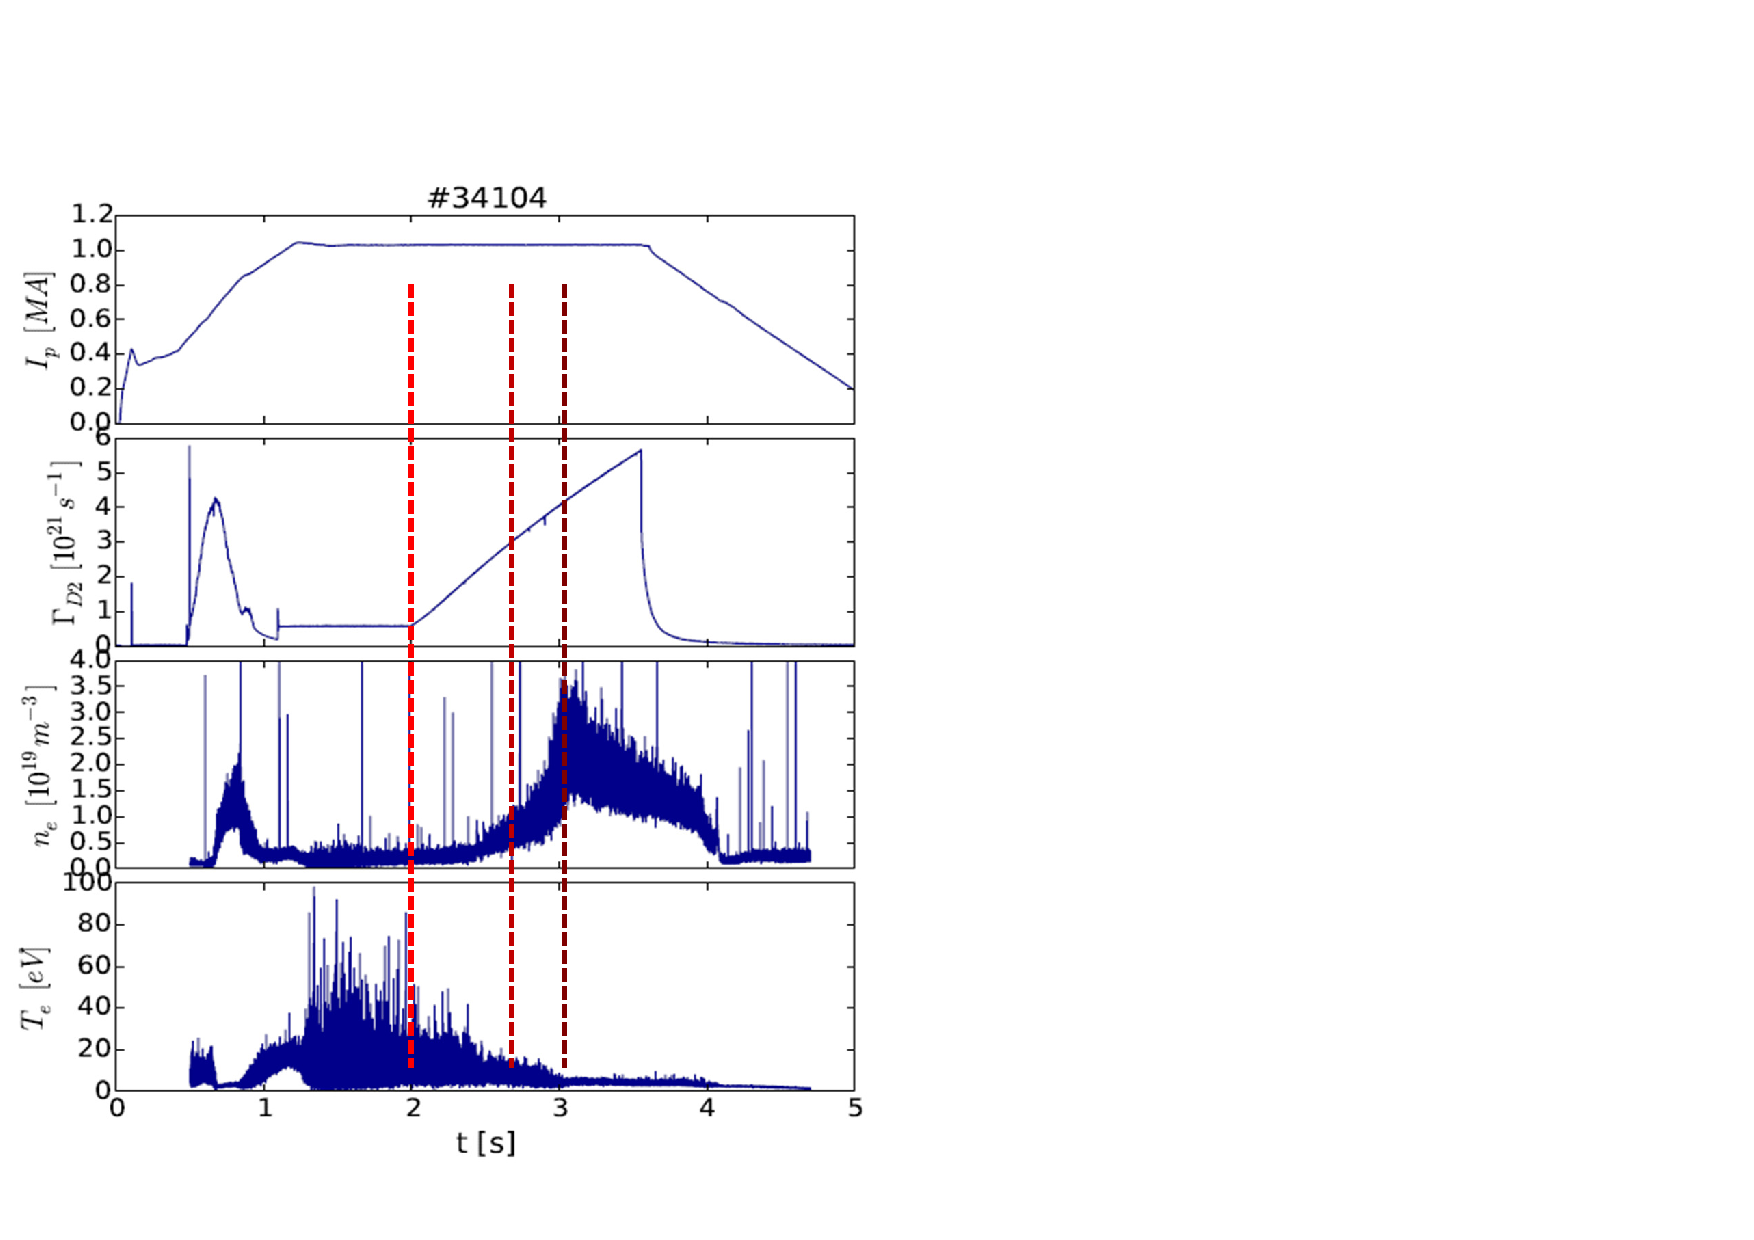
\includegraphics[width=\textwidth]{../../Experiments/AUG/analysis/pdfbox/Dalpha/Agostini_Fig1.pdf}
      \end{column}
    \end{columns}
  }
  \only<2>{
    \centering{\includgraphics[width=7cm]{../../Experiments/AUG/analysis/pdfbox/Dalpha/Agostini_Fig2.pdf}}
    At the beginning of the fueling ramp emission localized in the HFS
  }
  \only<3>{
    \centering{\includgraphics[width=7cm]{../../Experiments/AUG/analysis/pdfbox/Dalpha/Agostini_Fig3.pdf}}
Radiation starts moving along the separatrix with different patterns between the two radiation
  }
  \only<4>{
    \centering{\includgraphics[width=7cm]{../../Experiments/AUG/analysis/pdfbox/Dalpha/Agostini_Fig4.pdf}}
    Emission propagate also towards the LFS and moves towards the CFR
  }
\end{frame}

\begin{frame}{Heat transport and power balance: D. Carralero}
  \only<1>{
    \begin{columns}
    \begin{column}{0.5\textwidth}
      \begin{itemize}
        \item Using a large database (around 30 discharges) in
          L-Mode detailed ion and electron temperature profiles
          collected
        \item Consistent ion temperature drop observed whenever shoulder
          is observed
      \end{itemize}
    \end{column}
    \begin{column}{0.5\textwidth}
      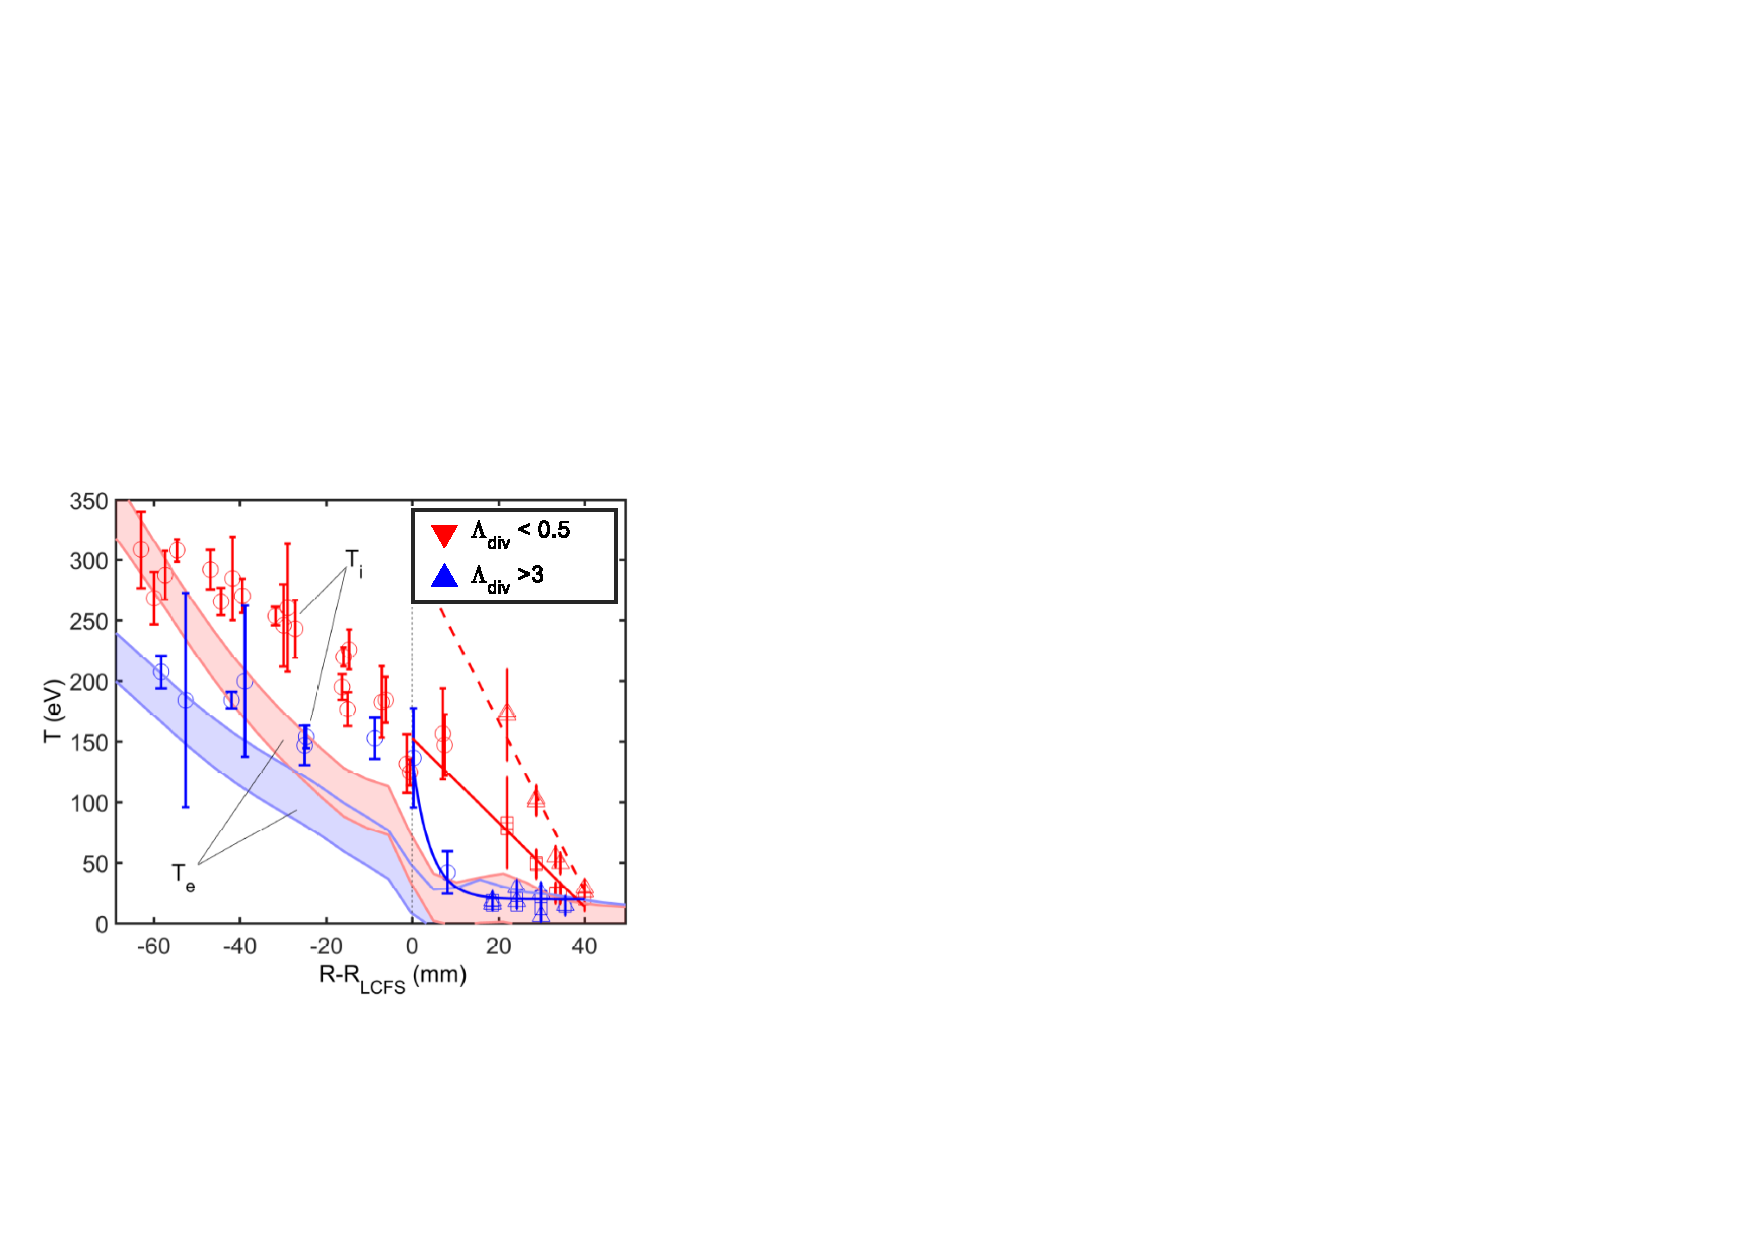
\includegraphics[width=\textwidth]{../../Experiments/AUG/analysis/pdfbox/Carralero_ionTemperature}
    \end{column}
  \end{columns}
}
\only<2>{
  \centering{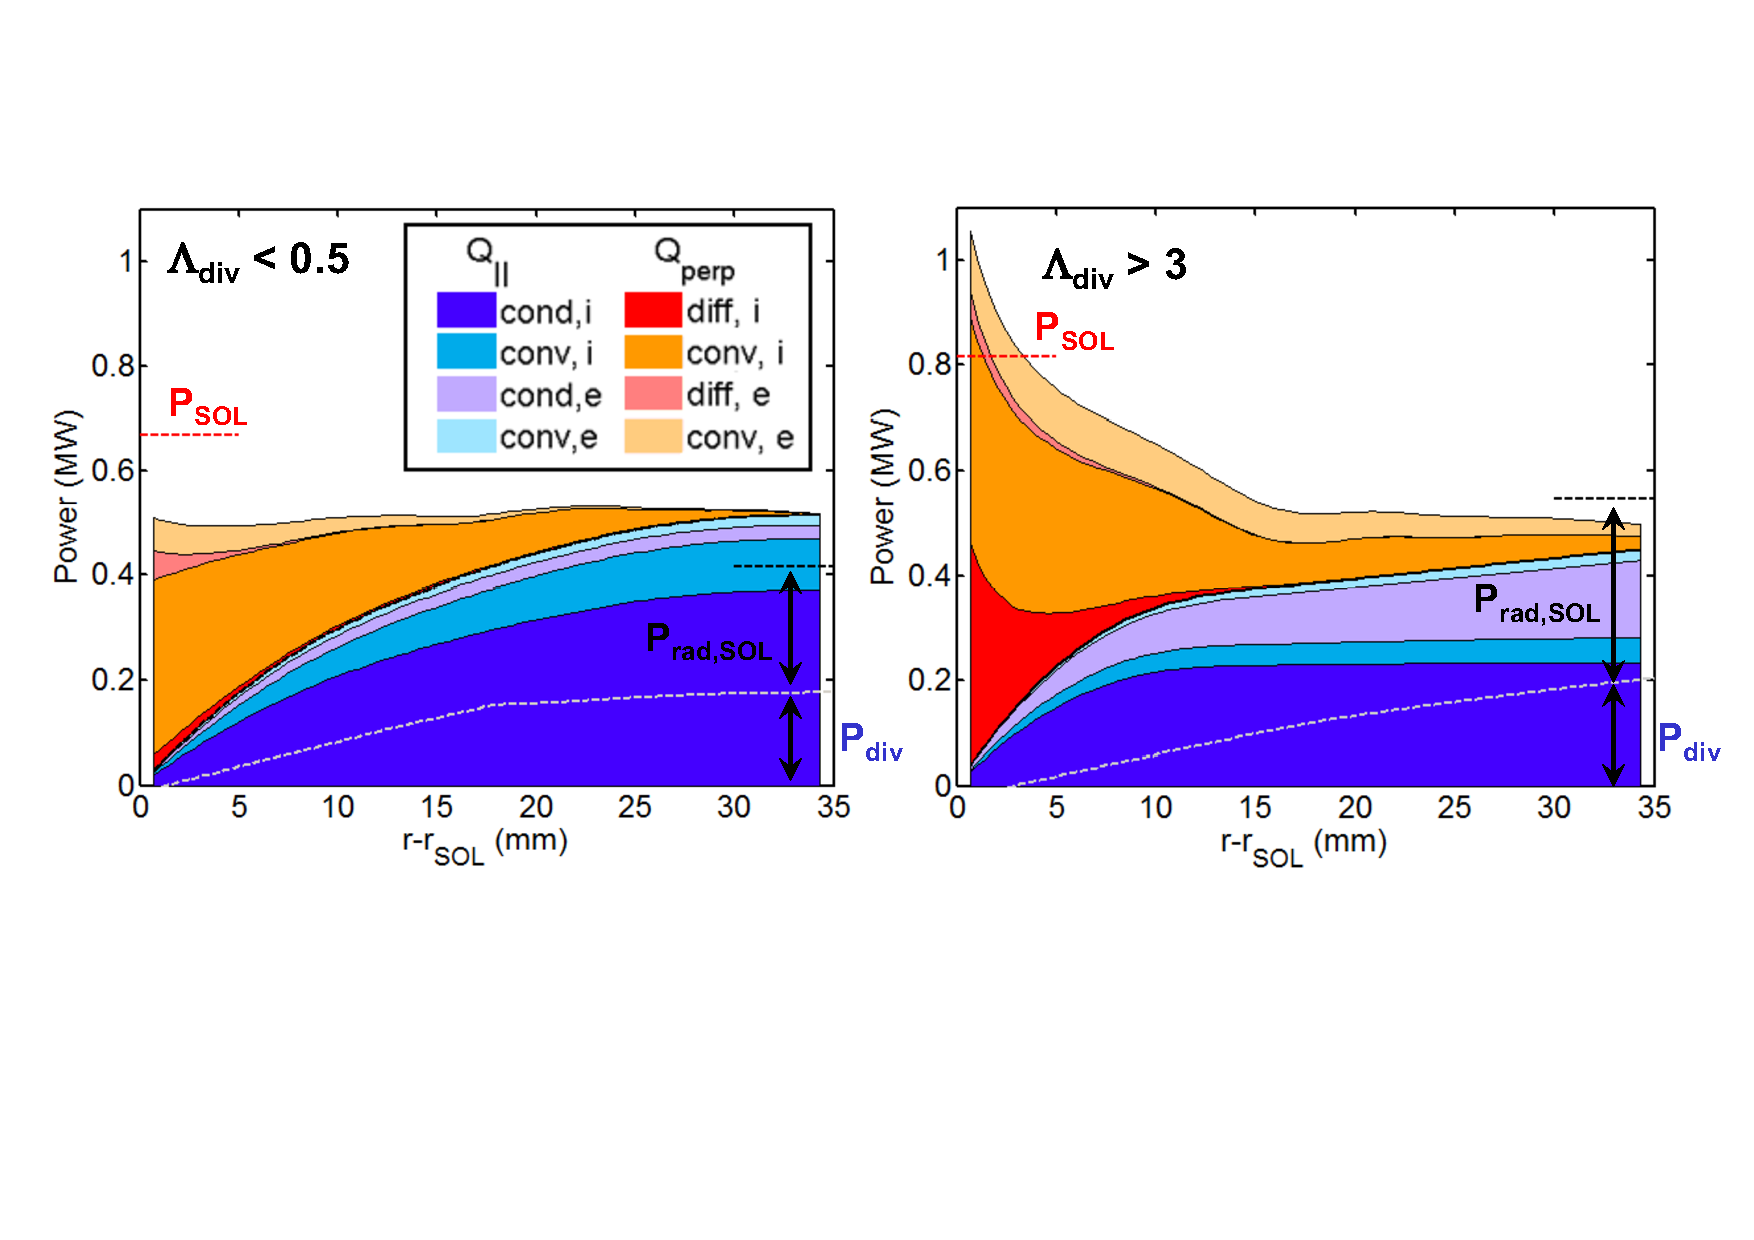
\includegraphics[width=7cm]{../../Experiments/AUG/analysis/pdfbox/Carralero_powerbalance}}
  \Fontvi
  \begin{itemize}
    \item Parallel heat flux dominated by ion conduction whereas
      perpendicular component dominated by ion convection
    \item In high density regime a substantial fraction of
      P$_{\mathrm{SOL}}$ still remains in the $Q_{\perp}$ for
      $r-r_{\mathrm{LCFS}} \sim 20$ cm
  \end{itemize}
}
\end{frame}
% % %% H-Mode same fueling
\begin{frame}{H-Mode analysis on AUG}
    \Fontvi
  \vspace{-1cm}
  \begin{columns}
  \begin{column}{0.55\textwidth}
    \centering{\includegraphics<1>[height=0.8\textheight]{../../Experiments/AUG/analysis/pdfbox/GeneralComparisonShot34276_34278_34281.pdf}}
    \centering{\includegraphics<2>[width=\textwidth]{../../Experiments/AUG/analysis/pdfbox/PuffingIpolsola34276_34278_34281}}
  \centering{\includegraphics<3>[height=0.75\textheight]{../../Experiments/AUG/analysis/pdfbox/UpstreamDivertorProfiles34276_34278_34281}}
  \centering{\includegraphics<4>[width=\textwidth]{../../Experiments/Comparison/pdfbox/EfoldSizeShots34276_34278}}
  \centering{\includegraphics<5>[width=\textwidth]{../../Experiments/Comparison/pdfbox/EfoldSizeShots34276_34278_34281}}
  \end{column}
  \begin{column}{0.45\textwidth}
    \begin{itemize}
    \item<1|only@1> We perform a series of shots in H-Mode with 6.5
      total heating power where we changed the fueling and the
      efficiency of cryopumps. Specifically we have
      \begin{itemize}
        \item<1|only@1>\textcolor{colorA}{\# 34276 without the
            cryompumps}
        \item<1|only@1> \textcolor{colorB}{\# 34278 with the same
            fueling as} \textcolor{colorA}{\# 34276} \textcolor{colorB}{but with the cryompump}
        \item<1|only@1> \textcolor{colorC}{\#34281 where we increase
            fueling and seeding trying to mimic the same subdivertor
            pressure as} \textcolor{colorA}{\# 34276}
      \end{itemize}
    \item<1|only@1> Keeping the same fueling with the cryopump clearly
      reduce the pressure in the the sub-divertor area, we don't reach
      clear detachment and the edge density is constant even during
      the fueling ramp. Degraded H-mode reached later without the cryopump
      
    \item<2|only@2> Different behavior of ELM during the fueling
      ramp. ELM size and frequency changes strongly without the
      cryopump or during extreme fueling case
    \item<3|only@3> The profiles for shot \# 34278 with the cryopum
      and lower fueling remains more steep in all the three timing
      wind and the plasma is still attached. Interestingly for shot \#
      34281 with the cryopumps and higher fueling the detachment is
      more pronounced
    \item<4|only@4> Without the cryopumps, we reached flatter
         profiles with comparable inter-ELM resolved blob-size. This
         indicates strong neutral pressure effects in determining
         upstream profiles
    \item<5|only@5> Increasing the fueling and correspondingly the
      divertor neutral pressure move towards a situation similar to
      \# 34276 without the cryopump
      \end{itemize}
  \end{column}
\end{columns}
\end{frame}

\begin{frame}{Conclusion}
  \Fontvi
  \begin{itemize}
    \item Current scan at constant B$_t$ and at constant q$_{95}$
      performed during density ramps L-Mode experiments both at AUG
      and TCV
    \item In both the case shoulder appear earlier in density at lower
      current but AUG shows reconciliation of behavior if considered
      as a function of greenwald fraction and $\Lambda_{div}$ for
      constant B$_t$ but not for constant q$_{95}$. AUG still well
      represented by $\Lambda_{div}$. \alert{Shoulder starts
        developing at the onset of highly recycling regime}
    \item Both the experiments exhibit at constant B$_t$ flattening of the profile as
      blob size is increasing, independently from the current. The
      same behavior is observed during current scan at constant
      q$_{95}$ \alert{only on AUG}
    \item On TCV during the current scan at constant q$_{95}$
      detachment not reached and this \alert{prevents upstream profile
        flattening}
    \item H-Mode experiments performed on AUG where fueling and
      pumping have been varied. \alert{Proved inter-ELM profile flattening
      also in H-Mode} \alert{but high neutral pressure (not only edge
      density) is needed}
  \item<2-> \textbf{\textcolor{ta3scarletred}{Can we find a different parameter to reconcile
        the experimental observation?}}
  \end{itemize}
\end{frame}

\begin{frame}{On going work}
  A series of works are still on-going \textcolor{ta3scarletred}{or
    yet to be started}
  \begin{itemize}[<+->]
    \item Neutral density estimate from light emission
      \textbf{M. Agostini}
    \item Wall embedded probe analysis \textbf{S. Costea,
        M. Spolaore}
    \item Shoulder from Reflectometry analysis \textbf{E. Seliunin}
    \item \textcolor{ta3scarletred}{SOLPS modelling AUG/TCV for modelling collisionality
      along flux tube and compare to measurement}
    \item \textcolor{ta3scarletred}{Balmer series analysis for
        recombination analysis on TCV \textbf{K. Verhaegh} and MSI for
      radiation front neutrals (?)}
    \item \textcolor{ta3orange}{GPI analysis and comparison with probe
      \textbf{N. Walkden, I. Cziegler}}  
  \item \textcolor{ta3scarletred}{HFSD}
    \item \textcolor{ta3scarletred}{\ldots}
  \end{itemize}
\end{frame}
\end{document}

